%---------------------------------------------------------------------
%
%                          Cap�tulo 4
%
%---------------------------------------------------------------------

\chapter{Metodolog�as utilizadas}

\begin{FraseCelebre}
	\begin{Frase}
		"Juntarse es un comienzo. Seguir juntos es un progreso. Trabajar juntos es un �xito". 
	\end{Frase}
	\begin{Fuente}
		Henry Ford
	\end{Fuente}
\end{FraseCelebre}


%-------------------------------------------------------------------
\section{Reuniones}
%-------------------------------------------------------------------
\label{cap4:sec:Reuniones}

Para una buena organizaci�n, desde el principio el equipo de trabajo se ha reunido una vez a la semana para asignar las diferentes tareas, comentar el trabajo realizado y poner en com�n todos los conocimientos adquiridos por cada uno. A lo largo de la semana tambi�n hab�a reuniones a trav�s de Skype\footnote {\url{https://www.skype.com/es/}} para comentar y resolver las posibles dudas que podr�an surgir durante el proceso. \\

El equipo tambi�n se ha mantenido en contacto v�a email con los tutores comentando el estado del proyecto. A esto se a�adieron reuniones mensuales con ellos para realizar correcciones de la memoria, revisar el progreso, resolver dudas y comentar las tareas necesarias para las siguientes fases.\\

De esta forma, los integrantes del equipo y los tutores han estado informados constantemente del progreso del trabajo, se ha podido hacer un reparto claro de tareas y se han podido establecer tiempos de entregas realistas y factibles.\\

%-------------------------------------------------------------------
\section{Trello}
%-------------------------------------------------------------------
\label{cap4:sec:Trello}

A lo largo de todo el proyecto se ha utilizado la herramienta Trello\footnote {\url{https://trello.com/}} para el reparto claro y equitativo de tareas entre los componentes del equipo de trabajo. Trello consiste en un conjunto de tableros, a los cuales se les pueden a�adir una serie de tareas con diferentes estados. Esto podemos observarlo en la Figura X, donde se muestra un ejemplo de tablero utilizado en el desarrollo del proyecto. Esta herramienta permite ver de manera sencilla el estado del proyecto, facilitando as� la organizaci�n de las tareas a realizar. En el desarrollo de ``Text2LSE'' se han utilizado tres tableros distintos:

\begin{itemize}
	
	\item \textbf{Investigaci�n:} Incluye las tareas relacionadas con toda la investigaci�n referente al proyecto, como por ejemplo LSE, Python, PLN, etc.
	
	\item \textbf{Desarrollo:} Este tablero contiene las distintas tareas de desarrollo de c�digo, tanto de la aplicaci�n web como de la API.
	
	\item \textbf{Memoria:} En este tablero se encuentran las distintas tareas relacionadas con el desarrollo y correcci�n de los apartados de la memoria.
	
\end{itemize}

Para una mayor organizaci�n, cada tablero se ha estructurado en tres estados:

\begin{itemize}
	
	\item \textbf{Lista de Tareas:} Lista de tareas asignadas a un miembro del equipo en concreto que todav�a est�n sin empezar.
	
	\item \textbf{En proceso:} Tareas que el propietario de la tarjeta tiene en proceso de desarrollo. 
	
	\item \textbf{Hecho:} Tareas completadas y subidas al repositorio de GitHub.
	
\end{itemize}

Cada miembro del equipo ha sido el encargado de actualizar en tiempo real el estado de las tarjetas que ten�a asignadas. De esta manera se ha conseguido tener una buena organizaci�n con respecto a las tareas a realizar.

%\begin{figure}[]
%	\centering
%	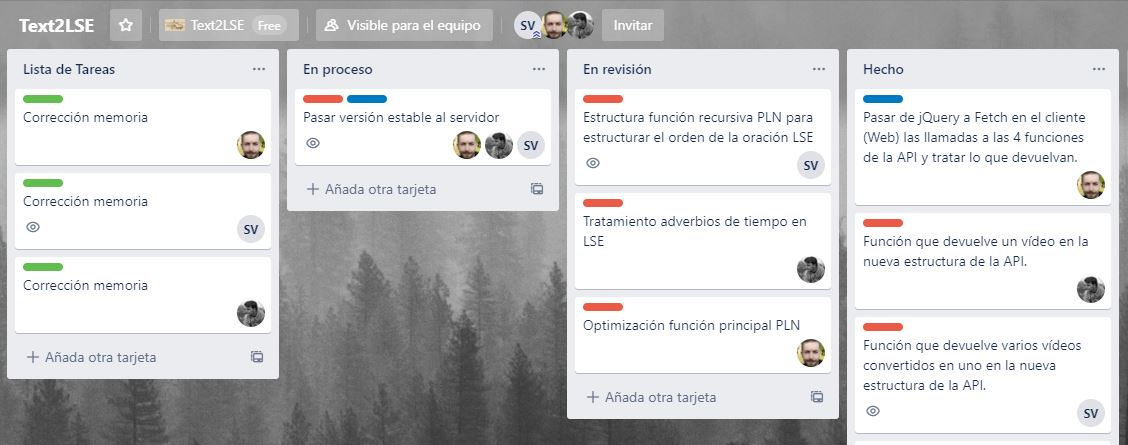
\includegraphics[width=1\textwidth]{Imagenes/Fuentes/Metodologias/trello.png}
%	\caption{Tablero \textit{``Memoria''} utilizado en el proyecto.  }
%	\label {fig: imgTrello}
%\end{figure}
% ~\ref {fig: imgTrello} -> elegir imagen de tablero

%-------------------------------------------------------------------
\section{Control de versiones}
%-------------------------------------------------------------------
\label{cap4:sec:Control de versiones}
\subsection{GIT}

Para el desarrollo del proyecto se ha utilizado Git \footnote{Web oficial de Git \url{https://git-scm.com/}} que es un sistema de control de versiones distribuido que sirve para trabajar en equipo de una manera muy sencilla y optimizada. Git permite al usuario tener un control absoluto de su proyecto pudiendo ver todos los cambios realizados en nuestra aplicaci�n y nuestro c�digo por cada uno de los miembros o incluso volver a versiones anteriores del proyecto.

Sus principales herramientas son:

\begin{itemize}
	
	\item \textbf{Repository:} es un directorio donde se almacenan los archivos de tu proyecto. Puede estar ubicado en el almacenamiento de GitHub o en un repositorio local en tu computadora y tenerlos sincronizados.
	
	
	\item \textbf{Branch:} es una copia de tu repositorio cuyo desarrollo es independiente al repositorio central u otras ramas. Una vez realizados los cambios se puede combinar tu rama con otras ramas y con el repositorio central mediante un request.
	 
	
	\item \textbf{Commits:} son los cambios realizados en los archivos de tu repositorio local.

	\item \textbf{Pull:} acci�n que actualiza el repositorio local de tu ordenador con la �ltima versi�n del proyecto alojado en Github.
	
	\item \textbf{Push:} permite subir a Github los commits realizados en el repositorio local.	
	
\end{itemize}


\subsection{GITHUB}
GitHub \footnote{Web oficial de Github \url{https://help.github.com/}} es una plataforma que proporciona una interfaz que mediante las herramientas del control de versiones Git permite ver y llevar el registro de todos los cambios realizados en nuestro proyecto, organizarlos y resolver cualquier conflicto que pueda surgir. \\

Github tambi�n funciona como una red social para desarrolladores ya que permite a otros usuarios ver y colaborar en tus repositorios as� como resolver dudas que se tengan.





